\textbf{Comparación de solución de tiempo continuo y solución de tiempo discreto utilizando funciones de transferencia para diferentes valores de tiempo de muestreo }

{\Large Control discreto de un sistema de tiempo continuo.}

Considere un sistema lineal e invariante en el tiempo representado por la siguiente función de transferencia

\begin{equation*}
	G(s)=\frac{1}{s(s+3)}
\end{equation*}

\begin{itemize}
	\item Determine la estabilidad del sistema.
Para poder determinar la estabilidad del sistema, vamos a ver con MATLAB en donde se encuentran sus Polos. Para ello vamos a escribir los siguientes comandos.\\


\begin{figure}[H]
	\centering
	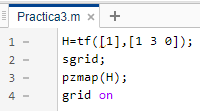
\includegraphics[scale=0.9]{cod1.png} \\
	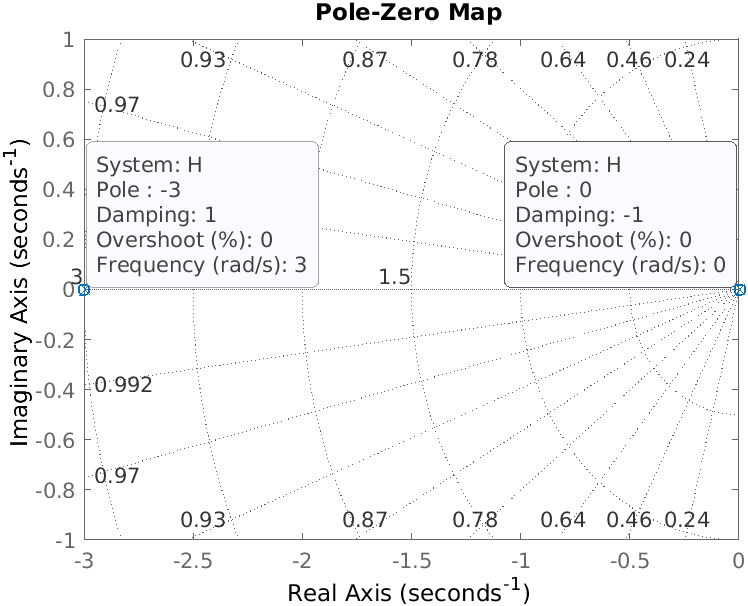
\includegraphics[scale=0.9]{G1.png}
	\caption{{Gráfica de polos y ceros}}
	\label{fig:salidaTs001-4}
\end{figure}

Como se puede ver un polo está en s=-3, pero el otro polo está en s=0, por lo que no podemos decir si el sistema es estable o no. Ya que para que un sistema sea estable TODOS sus polos deben de estar en la parte izquierda del plano S. Por lo que primero veremos su respuesta al escalón para así poder determinar si el sistema es estable o no.

	\item Utilizando el software especializado de su preferencia, determine la respuesta al escalón del sistema y describa como es su comportamiento.
Para determinar la respuesta al escalón del sistema vamos a agregar el siguiente comando al código anterior: step(H,'-')\\
 \\

\begin{figure}[H]
	\centering
	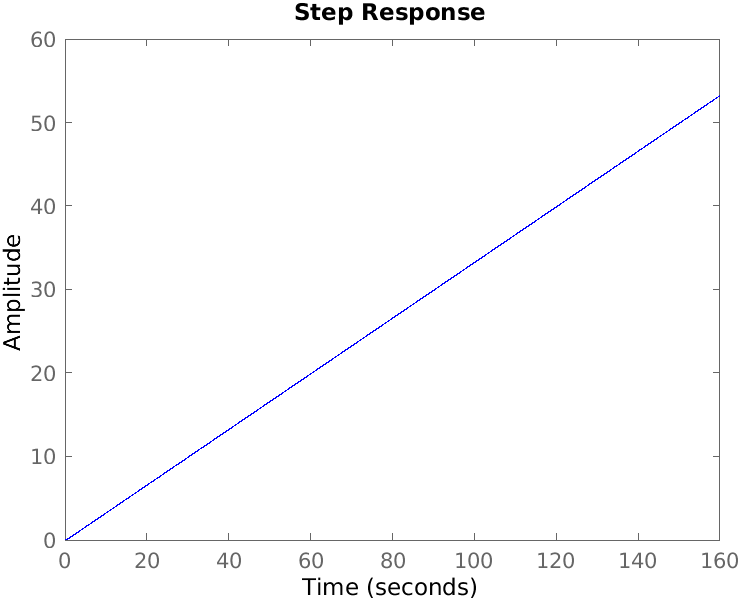
\includegraphics[scale=0.9]{G2.png}
	\caption{{Gráfica respuesta al escalón}}
	\label{fig:salidaTs001-5}
\end{figure}

Al analizar esta gráfica podemos ver que no tiene fin, en otras palabras, la gráfica no tiene límite, ya que solamente es creciente conforme va avanzando en el eje X positivo. Por lo que podemos concluir a la pregunta anterior que NO es estable el sistema.

\end{itemize}
